\documentclass[11pt,a4paper]{article}

\usepackage[margin=2.5cm]{geometry}
\usepackage{amsmath,amssymb,amsthm}
\usepackage{mathtools}
\usepackage{hyperref}
\usepackage{xcolor}
\usepackage{listings}
\usepackage{algorithm}
\usepackage{algpseudocode}
\usepackage{tikz}
\usetikzlibrary{arrows.meta,positioning,fit,shapes.geometric,shapes.multipart,
                decorations.pathreplacing,backgrounds,calc,shadows}
\usepackage{booktabs}
\usepackage{microtype}
\usepackage{enumitem}
\usepackage{float}
\usepackage{xspace}    	 % For new commands

\hypersetup{
  colorlinks=true,
  linkcolor=blue!70!black,
  citecolor=green!60!black,
  urlcolor=blue!80!black,
}

% ─── theorem environments ───────────────────────────────────────────────────
\newtheorem{definition}{Definition}[section]
\newtheorem{remark}{Remark}[section]
\newtheorem{lemma}{Lemma}[section]
\newtheorem{observation}{Observation}[section]

% ─── TikZ styles ────────────────────────────────────────────────────────────
\tikzset{
  node box/.style = {draw, rounded corners=3pt, minimum width=2.6cm,
                      minimum height=0.7cm, font=\small, align=center,
                      fill=white, },
  proof node/.style = {draw, circle, minimum size=1.1cm, font=\small,
                        align=center, fill=blue!10, drop shadow},
  leaf node/.style = {draw, circle, minimum size=.5cm, font=\scriptsize,
                        align=center, fill=green!10, drop shadow},
  thresh node/.style= {draw, diamond, minimum size=1.4cm, font=\scriptsize,
                        align=center, fill=orange!15, drop shadow,
                        inner sep=1pt, aspect=1.3},
  root box/.style   = {draw, rounded corners=4pt, minimum width=3cm,
                        minimum height=0.8cm, font=\small\bfseries, align=center,
                        fill=blue!10, drop shadow},
  arr/.style        = {-{Stealth[length=5pt]}, thick},
  dashed arr/.style = {-{Stealth[length=5pt]}, dashed, gray},
  hash arrow/.style = {-{Stealth[length=4pt]}, thick, blue!60},
}

% ─── colour macros ───────────────────────────────────────────────────────────
\definecolor{darkblue}{RGB}{0,70,127}
\definecolor{darkgreen}{RGB}{0,100,50}
\definecolor{darkorange}{RGB}{180,90,0}
\definecolor{darkred}{RGB}{150,20,20}

% ─── code listing style ─────────────────────────────────────────────────────
\lstdefinestyle{zkdsl}{
  language=Python,
  basicstyle=\ttfamily\scriptsize,
  keywordstyle=\color{darkblue}\bfseries,
  commentstyle=\color{darkgreen}\itshape,
  stringstyle=\color{darkorange},
, numbers=left%
, firstnumber=auto%
, numberblanklines=true%
, frame=trbL%
, numberstyle=\tiny%
, frame=leftline%
, numbersep=7pt%
, framesep=5pt%
, framerule=10pt%
, xleftmargin=15pt%
, backgroundcolor=\color[gray]{0.97}%
, rulecolor=\color[gray]{0.90}%
}

\lstdefinelanguage{Rust}{%
  sensitive%
, morecomment=[l]{//}%
, morecomment=[s]{/*}{*/}%
, moredelim=[s][{\itshape\color[rgb]{0,0,0.75}}]{\#[}{]}%
, morestring=[b]{"}%
, alsodigit={}%
, alsoother={}%
, alsoletter={!}%
%
%
% [1] reserve keywords
% [2] traits
% [3] primitive types
% [4] type and value constructors
% [5] identifier
%
, morekeywords={break, continue, else, for, if, in, loop, match, return, while}  % control flow keywords
, morekeywords={as, const, let, move, mut, ref, static}  % in the context of variables
, morekeywords={dyn, enum, fn, impl, Self, self, struct, trait, type, union, use, where}  % in the context of declarations
, morekeywords={crate, extern, mod, pub, super}  % in the context of modularisation
, morekeywords={unsafe}  % markers
, morekeywords={abstract, alignof, become, box, do, final, macro, offsetof, override, priv, proc, pure, sizeof, typeof, unsized, virtual, yield}  % reserved identifiers
%
% grep 'pub trait [A-Za-z][A-Za-z0-9]*' -r . | sed 's/^.*pub trait \([A-Za-z][A-Za-z0-9]*\).*/\1/g' | sort -u | tr '\n' ',' | sed 's/^\(.*\),$/{\1}\n/g' | sed 's/,/, /g'
, morekeywords=[2]{Add, AddAssign, Any, AsciiExt, AsInner, AsInnerMut, AsMut, AsRawFd, AsRawHandle, AsRawSocket, AsRef, Binary, BitAnd, BitAndAssign, Bitor, BitOr, BitOrAssign, BitXor, BitXorAssign, Borrow, BorrowMut, Boxed, BoxPlace, BufRead, BuildHasher, CastInto, CharExt, Clone, CoerceUnsized, CommandExt, Copy, Debug, DecodableFloat, Default, Deref, DerefMut, DirBuilderExt, DirEntryExt, Display, Div, DivAssign, DoubleEndedIterator, DoubleEndedSearcher, Drop, EnvKey, Eq, Error, ExactSizeIterator, ExitStatusExt, Extend, FileExt, FileTypeExt, Float, Fn, FnBox, FnMut, FnOnce, Freeze, From, FromInner, FromIterator, FromRawFd, FromRawHandle, FromRawSocket, FromStr, FullOps, FusedIterator, Generator, Hash, Hasher, Index, IndexMut, InPlace, Int, Into, IntoCow, IntoInner, IntoIterator, IntoRawFd, IntoRawHandle, IntoRawSocket, IsMinusOne, IsZero, Iterator, JoinHandleExt, LargeInt, LowerExp, LowerHex, MetadataExt, Mul, MulAssign, Neg, Not, Octal, OpenOptionsExt, Ord, OsStrExt, OsStringExt, Packet, PartialEq, PartialOrd, Pattern, PermissionsExt, Place, Placer, Pointer, Product, Put, RangeArgument, RawFloat, Read, Rem, RemAssign, Seek, Shl, ShlAssign, Shr, ShrAssign, Sized, SliceConcatExt, SliceExt, SliceIndex, Stats, Step, StrExt, Sub, SubAssign, Sum, Sync, TDynBenchFn, Terminal, Termination, ToOwned, ToSocketAddrs, ToString, Try, TryFrom, TryInto, UnicodeStr, Unsize, UpperExp, UpperHex, WideInt, Write}
, morekeywords=[2]{Send}  % additional traits
%
, morekeywords=[3]{bool, char, f32, f64, i8, i16, i32, i64, isize, str, u8, u16, u32, u64, unit, usize, i128, u128}  % primitive types
%
, morekeywords=[4]{Err, false, None, Ok, Some, true}  % prelude value constructors
% grep 'pub \(type\|struct\|enum\) [A-Za-z][A-Za-z0-9]*' -r . | sed 's/^.*pub \(type\|struct\|enum\) \([A-Za-z][A-Za-z0-9]*\).*/\2/g' | sort -u | tr '\n' ',' | sed 's/^\(.*\),$/{\1}\n/g' | sed 's/,/, /g'    
, morekeywords=[3]{AccessError, Adddf3, AddI128, AddoI128, AddoU128, ADDRESS, ADDRESS64, addrinfo, ADDRINFOA, AddrParseError, Addsf3, AddU128, advice, aiocb, Alignment, AllocErr, AnonPipe, Answer, Arc, Args, ArgsInnerDebug, ArgsOs, Argument, Arguments, ArgumentV1, Ashldi3, Ashlti3, Ashrdi3, Ashrti3, AssertParamIsClone, AssertParamIsCopy, AssertParamIsEq, AssertUnwindSafe, AtomicBool, AtomicPtr, Attr, auxtype, auxv, BackPlace, BacktraceContext, Barrier, BarrierWaitResult, Bencher, BenchMode, BenchSamples, BinaryHeap, BinaryHeapPlace, blkcnt, blkcnt64, blksize, BOOL, boolean, BOOLEAN, BoolTrie, BorrowError, BorrowMutError, Bound, Box, bpf, BTreeMap, BTreeSet, Bucket, BucketState, Buf, BufReader, BufWriter, Builder, BuildHasherDefault, BY, BYTE, Bytes, CannotReallocInPlace, cc, Cell, Chain, CHAR, CharIndices, CharPredicateSearcher, Chars, CharSearcher, CharsError, CharSliceSearcher, CharTryFromError, Child, ChildPipes, ChildStderr, ChildStdin, ChildStdio, ChildStdout, Chunks, ChunksMut, ciovec, clock, clockid, Cloned, cmsgcred, cmsghdr, CodePoint, Color, ColorConfig, Command, CommandEnv, Component, Components, CONDITION, condvar, Condvar, CONSOLE, CONTEXT, Count, Cow, cpu, CRITICAL, CStr, CString, CStringArray, Cursor, Cycle, CycleIter, daddr, DebugList, DebugMap, DebugSet, DebugStruct, DebugTuple, Decimal, Decoded, DecodeUtf16, DecodeUtf16Error, DecodeUtf8, DefaultEnvKey, DefaultHasher, dev, device, Difference, Digit32, DIR, DirBuilder, dircookie, dirent, dirent64, DirEntry, Discriminant, DISPATCHER, Display, Divdf3, Divdi3, Divmoddi4, Divmodsi4, Divsf3, Divsi3, Divti3, dl, Dl, Dlmalloc, Dns, DnsAnswer, DnsQuery, dqblk, Drain, DrainFilter, Dtor, Duration, DwarfReader, DWORD, DWORDLONG, DynamicLibrary, Edge, EHAction, EHContext, Elf32, Elf64, Empty, EmptyBucket, EncodeUtf16, EncodeWide, Entry, EntryPlace, Enumerate, Env, epoll, errno, Error, ErrorKind, EscapeDebug, EscapeDefault, EscapeUnicode, event, Event, eventrwflags, eventtype, ExactChunks, ExactChunksMut, EXCEPTION, Excess, ExchangeHeapSingleton, exit, exitcode, ExitStatus, Failure, fd, fdflags, fdsflags, fdstat, ff, fflags, File, FILE, FileAttr, filedelta, FileDesc, FilePermissions, filesize, filestat, FILETIME, filetype, FileType, Filter, FilterMap, Fixdfdi, Fixdfsi, Fixdfti, Fixsfdi, Fixsfsi, Fixsfti, Fixunsdfdi, Fixunsdfsi, Fixunsdfti, Fixunssfdi, Fixunssfsi, Fixunssfti, Flag, FlatMap, Floatdidf, FLOATING, Floatsidf, Floatsisf, Floattidf, Floattisf, Floatundidf, Floatunsidf, Floatunsisf, Floatuntidf, Floatuntisf, flock, ForceResult, FormatSpec, Formatted, Formatter, Fp, FpCategory, fpos, fpos64, fpreg, fpregset, FPUControlWord, Frame, FromBytesWithNulError, FromUtf16Error, FromUtf8Error, FrontPlace, fsblkcnt, fsfilcnt, fsflags, fsid, fstore, fsword, FullBucket, FullBucketMut, FullDecoded, Fuse, GapThenFull, GeneratorState, gid, glob, glob64, GlobalDlmalloc, greg, group, GROUP, Guard, GUID, Handle, HANDLE, Handler, HashMap, HashSet, Heap, HINSTANCE, HMODULE, hostent, HRESULT, id, idtype, if, ifaddrs, IMAGEHLP, Immut, in, in6, Incoming, Infallible, Initializer, ino, ino64, inode, input, InsertResult, Inspect, Instant, int16, int32, int64, int8, integer, IntermediateBox, Internal, Intersection, intmax, IntoInnerError, IntoIter, IntoStringError, intptr, InvalidSequence, iovec, ip, IpAddr, ipc, Ipv4Addr, ipv6, Ipv6Addr, Ipv6MulticastScope, Iter, IterMut, itimerspec, itimerval, jail, JoinHandle, JoinPathsError, KDHELP64, kevent, kevent64, key, Key, Keys, KV, l4, LARGE, lastlog, launchpad, Layout, Lazy, lconv, Leaf, LeafOrInternal, Lines, LinesAny, LineWriter, linger, linkcount, LinkedList, load, locale, LocalKey, LocalKeyState, Location, lock, LockResult, loff, LONG, lookup, lookupflags, LookupHost, LPBOOL, LPBY, LPBYTE, LPCSTR, LPCVOID, LPCWSTR, LPDWORD, LPFILETIME, LPHANDLE, LPOVERLAPPED, LPPROCESS, LPPROGRESS, LPSECURITY, LPSTARTUPINFO, LPSTR, LPVOID, LPWCH, LPWIN32, LPWSADATA, LPWSAPROTOCOL, LPWSTR, Lshrdi3, Lshrti3, lwpid, M128A, mach, major, Map, mcontext, Metadata, Metric, MetricMap, mflags, minor, mmsghdr, Moddi3, mode, Modsi3, Modti3, MonitorMsg, MOUNT, mprot, mq, mqd, msflags, msghdr, msginfo, msglen, msgqnum, msqid, Muldf3, Mulodi4, Mulosi4, Muloti4, Mulsf3, Multi3, Mut, Mutex, MutexGuard, MyCollection, n16, NamePadding, NativeLibBoilerplate, nfds, nl, nlink, NodeRef, NoneError, NonNull, NonZero, nthreads, NulError, OccupiedEntry, off, off64, oflags, Once, OnceState, OpenOptions, Option, Options, OptRes, Ordering, OsStr, OsString, Output, OVERLAPPED, Owned, Packet, PanicInfo, Param, ParseBoolError, ParseCharError, ParseError, ParseFloatError, ParseIntError, ParseResult, Part, passwd, Path, PathBuf, PCONDITION, PCONSOLE, Peekable, PeekMut, Permissions, PhantomData, pid, Pipes, PlaceBack, PlaceFront, PLARGE, PoisonError, pollfd, PopResult, port, Position, Powidf2, Powisf2, Prefix, PrefixComponent, PrintFormat, proc, Process, PROCESS, processentry, protoent, PSRWLOCK, pthread, ptr, ptrdiff, PVECTORED, Queue, radvisory, RandomState, Range, RangeFrom, RangeFull, RangeInclusive, RangeMut, RangeTo, RangeToInclusive, RawBucket, RawFd, RawHandle, RawPthread, RawSocket, RawTable, RawVec, Rc, ReadDir, Receiver, recv, RecvError, RecvTimeoutError, ReentrantMutex, ReentrantMutexGuard, Ref, RefCell, RefMut, REPARSE, Repeat, Result, Rev, Reverse, riflags, rights, rlim, rlim64, rlimit, rlimit64, roflags, Root, RSplit, RSplitMut, RSplitN, RSplitNMut, RUNTIME, rusage, RwLock, RWLock, RwLockReadGuard, RwLockWriteGuard, sa, SafeHash, Scan, sched, scope, sdflags, SearchResult, SearchStep, SECURITY, SeekFrom, segment, Select, SelectionResult, sem, sembuf, send, Sender, SendError, servent, sf, Shared, shmatt, shmid, ShortReader, ShouldPanic, Shutdown, siflags, sigaction, SigAction, sigevent, sighandler, siginfo, Sign, signal, signalfd, SignalToken, sigset, sigval, Sink, SipHasher, SipHasher13, SipHasher24, size, SIZE, Skip, SkipWhile, Slice, SmallBoolTrie, sockaddr, SOCKADDR, sockcred, Socket, SOCKET, SocketAddr, SocketAddrV4, SocketAddrV6, socklen, speed, Splice, Split, SplitMut, SplitN, SplitNMut, SplitPaths, SplitWhitespace, spwd, SRWLOCK, ssize, stack, STACKFRAME64, StartResult, STARTUPINFO, stat, Stat, stat64, statfs, statfs64, StaticKey, statvfs, StatVfs, statvfs64, Stderr, StderrLock, StderrTerminal, Stdin, StdinLock, Stdio, StdioPipes, Stdout, StdoutLock, StdoutTerminal, StepBy, String, StripPrefixError, StrSearcher, subclockflags, Subdf3, SubI128, SuboI128, SuboU128, subrwflags, subscription, Subsf3, SubU128, Summary, suseconds, SYMBOL, SYMBOLIC, SymmetricDifference, SyncSender, sysinfo, System, SystemTime, SystemTimeError, Take, TakeWhile, tcb, tcflag, TcpListener, TcpStream, TempDir, TermInfo, TerminfoTerminal, termios, termios2, TestDesc, TestDescAndFn, TestEvent, TestFn, TestName, TestOpts, TestResult, Thread, threadattr, threadentry, ThreadId, tid, time, time64, timespec, TimeSpec, timestamp, timeval, timeval32, timezone, tm, tms, ToLowercase, ToUppercase, TraitObject, TryFromIntError, TryFromSliceError, TryIter, TryLockError, TryLockResult, TryRecvError, TrySendError, TypeId, U64x2, ucontext, ucred, Udivdi3, Udivmoddi4, Udivmodsi4, Udivmodti4, Udivsi3, Udivti3, UdpSocket, uid, UINT, uint16, uint32, uint64, uint8, uintmax, uintptr, ulflags, ULONG, ULONGLONG, Umoddi3, Umodsi3, Umodti3, UnicodeVersion, Union, Unique, UnixDatagram, UnixListener, UnixStream, Unpacked, UnsafeCell, UNWIND, UpgradeResult, useconds, user, userdata, USHORT, Utf16Encoder, Utf8Error, Utf8Lossy, Utf8LossyChunk, Utf8LossyChunksIter, utimbuf, utmp, utmpx, utsname, uuid, VacantEntry, Values, ValuesMut, VarError, Variables, Vars, VarsOs, Vec, VecDeque, vm, Void, WaitTimeoutResult, WaitToken, wchar, WCHAR, Weak, whence, WIN32, WinConsole, Windows, WindowsEnvKey, winsize, WORD, Wrapping, wrlen, WSADATA, WSAPROTOCOL, WSAPROTOCOLCHAIN, Wtf8, Wtf8Buf, Wtf8CodePoints, xsw, xucred, Zip, zx}
%
, morekeywords=[5]{assert!, assert_eq!, assert_ne!, cfg!, column!, compile_error!, concat!, concat_idents!, debug_assert!, debug_assert_eq!, debug_assert_ne!, env!, eprint!, eprintln!, file!, format!, format_args!, include!, include_bytes!, include_str!, line!, module_path!, option_env!, panic!, print!, println!, select!, stringify!, thread_local!, try!, unimplemented!, unreachable!, vec!, write!, writeln!}  % prelude macros
}%

\lstdefinestyle{colouredRust}%
{ basicstyle=\ttfamily\small%
, identifierstyle=%
, commentstyle=\color[gray]{0.4}%
, stringstyle=\color[rgb]{0, 0, 0.5}%
, keywordstyle=\bfseries% reserved keywords
, keywordstyle=[2]\color[rgb]{0.75, 0, 0}% traits
, keywordstyle=[3]\color[rgb]{0, 0.5, 0}% primitive types
, keywordstyle=[4]\color[rgb]{0, 0.5, 0}% type and value constructors
, keywordstyle=[5]\color[rgb]{0, 0, 0.75}% macros
, columns=spaceflexible%
, keepspaces=true%
, showspaces=false%
, showtabs=false%
, showstringspaces=true%
}%

\lstdefinestyle{boxed}{
  style=colouredRust%
, numbers=left%
, firstnumber=auto%
, numberblanklines=true%
, frame=trbL%
, numberstyle=\tiny%
, frame=leftline%
, numbersep=7pt%
, framesep=5pt%
, framerule=10pt%
, xleftmargin=15pt%
, backgroundcolor=\color[gray]{0.97}%
, rulecolor=\color[gray]{0.90}%
}
% ─── short-hands ─────────────────────────────────────────────────────────────
\newcommand{\F}{\mathbb{F}}
\newcommand{\KB}{\mathbb{F}_{p}}  % KoalaBear base field
\newcommand{\KBext}{\mathbb{F}_{p^5}}
\newcommand{\hash}{\mathcal{H}}
\newcommand{\WOTS}{\textsf{WOTS}^{+}\xspace}
\newcommand{\aggsig}{\texttt{AggregatedSig}\xspace}
\newcommand{\bls}{\textsf{BLS12-381}\xspace}
\newcommand{\XMSS}{\textsf{XMSS}\xspace}
\newcommand{\hypertree}{\mathcal{T}}
\newcommand{\poseidon}{\textsf{Poseidon2}\xspace}
\newcommand{\WHIR}{\textsf{WHIR}\xspace}
\newcommand{\leanVM}{\textsf{leanVM}\xspace}
\newcommand{\leanProver}{\textsf{leanProver}\xspace}
\newcommand{\leanConsensus}{\textsf{leanConsensus}\xspace}
\newcommand{\Air}{\textsf{AIR}\xspace}

\title{%
  \textbf{Towards Distributed Validators on leanConsensus}\\[4pt]
}
\author{%
DV Labs
}
\date{February 2026}

\begin{document}
\maketitle
%\tableofcontents
%\newpage

% ═══════════════════════════════════════════════════════════════════════════════
\section{Introduction}
\label{sec:intro}
% ═══════════════════════════════════════════════════════════════════════════════

Ethereum's transition to proof-of-stake introduces a critical dependency on \emph{validator signatures}: every attestation and block proposal must be signed by an authorised validator.
The consensus layer currently relies on \bls for its native support for signatures aggregation.
However, on the quantum horizon, \bls signatures will be broken by Shor's algorithm running on a cryptographically-relevant quantum computer (CRQC).
To address this issue, the Beacon chain is being redesigned as \leanConsensus. Its core component is a hash-based zkVM aggregation system designed to address both the \emph{post-quantum} and the \emph{aggregation efficiency} requirements simultaneously. Its core contributions are:
\begin{enumerate}[label=(\roman*)]
  \item A Cairo-inspired zkVM (\leanVM) whose execution traces are proven by a \WHIR-based SNARK.
  \item An aggregation circuit defined in a domain-specific language (DSL) that can aggregate arbitrarily many $\XMSS$ signatures in a single succinct proof via a hierarchical tree of sub-proofs.
\end{enumerate}
This document provides an overview of \leanConsensus, with particular focus on how it can be extended to support threshold signatures, and what open engineering challenges remain for distributed validator (DV) solutions.

% ═══════════════════════════════════════════════════════════════════════════════
\section{Architecture of leanConsensus}
\label{sec:architecture}
% ═══════════════════════════════════════════════════════════════════════════════

\subsection{Cryptographic Primitives}
\label{subsec:primitives}

\paragraph{Base field.}
All arithmetic is performed over the \emph{KoalaBear} prime field $\F_{p}$ with $p = 2^{31} - 2^{24} + 1$ (a 31-bit prime with $2$-adicity 24). The extension used for polynomial commitments is $\F_{p^5}$, a degree-5 extension, giving a security level of 123 bits under the Johnson bound and 128 bits conjectured under the capacity bound. Every field element is 31 bits; an 8-element ``digest'' (the unit of hash output used throughout) is $31 \times 8 = 248$ bits.

\paragraph{Hash function.}
$\poseidon$ with a 16-element ($16 \times 31 = 496$-bit) state is used everywhere using the compression mode as it builds all Merkle trees in the system.  $\poseidon$ is algebraically friendly so that it integrates naturally into the AIR/Logup constraint system.

\paragraph{WOTS$^+$ one-time signatures.}
$\WOTS$ is the leaf-level signing primitive.
%The parameters used are:
%\begin{center}
%\begin{tabular}{ll}
%\toprule
%Parameter & Value \\ \midrule
%$V$ (number of hash chains) & 42 \\
%$W$ (Winternitz parameter) & 3 (chain length $2^W = 8$) \\
%$V_{\text{grind}}$ (grinding chains) & 2 \\
%Target sum $T$ & $V(L-1) - N_{\text{hashes}}$ \\
%Randomness length & 7 field elements \\
%Message length & 9 field elements \\
%\bottomrule
%\end{tabular}
%\end{center}
A $\WOTS$ private key $\mathsf{sk}_i = (s_1, \ldots, s_V) \in \KB^{V \cdot 8}$ generates a public key by iterating $\poseidon$ along each chain.  To sign, the hash encoding of the message is decomposed into per-chain lengths $e_1, \ldots, e_V$ with $\sum e_i = T$, and each chain tip is revealed at position $e_i$ from the start.

\paragraph{XMSS signatures.}
An $\XMSS$ key pair covers a lifetime of $2^{n}$ Ethereum \emph{slots} where $n$ is fixed at key generation time. The public key is a single digest $r_{\text{root}} \in \KB^8$
representing the root of a Merkle tree of depth $n$ over all $\WOTS$ leaf hashes.
A signature at slot $s$ consists of:
\begin{itemize}
  \item The $\WOTS$ randomness (7 field elements).
  \item $V$ chain tips ($V \times 8$ field elements).
  \item A Merkle authentication path of depth $n$ ($n \times 8$ field elements).
\end{itemize}

\subsection{The leanVM Execution Model}
\label{subsec:vm}

\leanVM is a register-free, memory-based virtual machine inspired by Cairo~\cite{cryptoeprint:2021/1063}. Its memory model is \emph{write-once}: each address can be written at most once;
a second write to the same address triggers a constraint violation. This property is central to correctness proofs. The instruction set includes:
\begin{itemize}[noitemsep]
  \item \textbf{Arithmetic}: \texttt{ADD}, \texttt{MUL} over $\KB$ and $\KBext$.
  \item \textbf{Memory}: load from and write to the write-once memory.
  \item \textbf{Control flow}: unconditional and conditional jumps; the program
        counter advances monotonically, enabling efficient AIR constraints.
  \item \textbf{Precompiles}: \texttt{poseidon16} and dot-product accelerators.
\end{itemize}

The execution trace is a table with three sub-tables: the \emph{Execution table} (instruction columns + runtime witness columns), the \emph{DotProduct table}, and the \emph{Poseidon16 table}.  The three tables are connected via the \emph{Logup bus}: each precompile call inserts a (fingerprinted) row into the corresponding table, and the Logup argument~\cite{cryptoeprint:2022/1530} proves that the multisets match.

\subsection{Proving Pipeline}
\label{subsec:proving}

\begin{figure}[H]
\centering
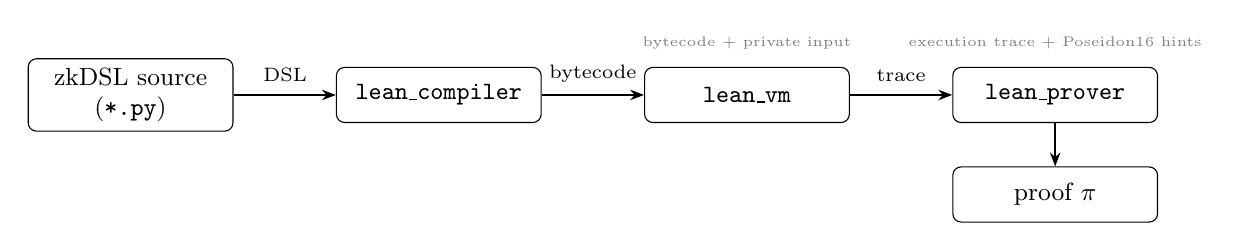
\begin{tikzpicture}[node distance=0.55cm and 1.3cm, align=center]
  \node[node box]  (dsl)   {zkDSL source\\(\texttt{*.py})};
  \node[node box, right=of dsl]   (cmp)   {\texttt{lean\_compiler}};
  \node[node box, right=of cmp]   (vm)    {\texttt{lean\_vm}};
  \node[node box, right=of vm]  (prv)   {\texttt{lean\_prover}};
  \node[node box, below=of prv] (out)   {proof $\pi$};

  \draw[arr] (dsl) --node [text width=2.5cm,midway,above=.1em ] {\scriptsize{DSL}} (cmp);
  \draw[arr] (cmp) --node [text width=1.5cm,midway,above=.1em ] {\scriptsize{bytecode}} (vm);
  \draw[arr] (vm)  --node [text width=1.5cm,midway,above=.1em ] {\scriptsize{trace}} (prv);
  \draw[arr] (prv) -- (out);

  \node[font=\tiny, gray, above=0.1cm of vm]  {bytecode + private input};
  \node[font=\tiny, gray, above=0.1cm of prv] {execution trace + Poseidon16 hints};
\end{tikzpicture}
\caption{Proving pipeline}
\label{fig:pipeline}
\end{figure}

\paragraph{SuperSpartan.}
The main proof system is a variant of Spartan~\cite{10.1007/978-3-030-56877-1_25} operating over extension field multilinear polynomials. The execution table's correctness is expressed as a sum over the Boolean hypercube of a degree-3 polynomial; a single sumcheck invocation reduces it to a point evaluation.

\paragraph{WHIR.}
Polynomial commitment proofs are generated with WHIR~\cite{10.1007/978-3-031-91134-7_8},
a Reed--Solomon proximity protocol with:
\begin{itemize}[noitemsep]
  \item Initial folding factor 7, subsequent factor 5.
  \item 18 grinding bits (proof-of-work).
  \item Code rate $\rho \in \{1/2, 1/4\}$ selectable per node.
\end{itemize}

\paragraph{Logup.}
The lookup argument connecting the three tables follows the \emph{logarithmic derivative} technique~\cite{cryptoeprint:2022/1530}.
The bus value is a linear combination of the table row, fingerprinted with Fiat-Shamir challenges.

\subsection{Aggregation Tree Topology}
\label{subsec:topology}

A single \leanConsensus node aggregates at most one ``level'' of the tree. Each node's circuit (\texttt{main.py}) handles two source types:

\begin{enumerate}
  \item \textbf{Raw XMSS} — individual validators signing directly.
  \item \textbf{Recursive children} — previously-proven aggregation nodes whose proofs are verified inside this node's circuit.
\end{enumerate}

The public state of a node is an \texttt{AggregatedSigs} structure:
\begin{itemize}[noitemsep]
  \item A list of public keys ($8 \times n$ field elements).
  \item A proof $\pi$ (a few hundred KiB, constant regardless of $n$).
  \item A \emph{bytecode claim} (an evaluation of the bytecode multilinear at a random point), used for recursive verification.
\end{itemize}

The global public key set is a deduplicated, sorted union of all raw and child public keys. Its \emph{Poseidon-slice-hash} (i.e., the running hash obtained by sequentially hashing consecutive pairs of pubkey digests) is committed in the proof's public input.

\paragraph{Bytecode claim reduction.}
When a node has $n_r$ recursive children, it must prove that each child was proved with the same bytecode.
The $2n_r$ bytecode claims (one per child,times two for the two halves of the recursion check) are collapsed into a single evaluation via a random linear combination and a sumcheck over the bytecode multilinear polynomial.
The resulting evaluation point is propagated to the parent node.

% ═══════════════════════════════════════════════════════════════════════════════
\section{Threshold Hash-Based Signatures}
\label{sec:threshold}
% ═══════════════════════════════════════════════════════════════════════════════

\subsection{Motivation: Distributed Validators}

In Ethereum's Distributed Validator (DV) model~\cite{DVT}, a single logical validator is operated by a cluster of $n$ independent nodes.
This architecture merges threshold cryptography with Byzantine Fault Tolerant (BFT) consensus to eliminate single points of failure, optimize uptime, and prevent equivocation.

\paragraph{DKG and threshold signatures.}
Rather than relying on a trusted dealer to generate and distribute the private signing key, which would represent a central point of failure, the cluster performs a Distributed Key Generation (DKG) protocol.
This allows the $n$ operators to collectively compute a public verification key while each operator strictly learns only their secret share.
In the pre-quantum BLS-based DV setting, the private signing key is split amongst multiple parties using a linear secret sharing scheme.
To produce a threshold \bls signature, a signer signs the agreed-upon data with its key share.
Because of the homomorphic properties unique to pairing-based schemes, k partial BLS signatures can be linearly combined into a single valid BLS signature that is indistinguishable from a standard, non-threshold signature.

\paragraph{Intra-cluster consensus and BFT.}
While threshold cryptography dictates \textit{how} a signature is constructed, it does not dictate \textit{what} is signed.
Before any partial signatures are generated, the $n$ nodes must run a BFT consensus protocol (e.g., an Istanbul BFT variant) to deterministically agree on the exact Beacon Chain duty (block or attestation data) they will execute.
By enforcing consensus prior to signing, the DV guarantees that no honest operator will sign conflicting data, effectively eliminating the risk of accidental slashing.

\paragraph{System guarantees and threshold parameters.}
To tolerate malicious (Byzantine) actors within the cluster, the system parameters are typically bound by the BFT threshold $n \geq 3f+1$, where $f$ is the maximum number of Byzantine nodes.
Consequently, the cryptographic signing threshold $k$ is usually set to $k \geq 2f+1$ (often represented as $k = \lceil \frac{2n}{3} \rceil$).


\paragraph{Impractical indistinguishable threshold hash-based signatures.}
Because the \textsf{BLS} homomorphic property abovementioned is unique to pairing-based schemes and does not transfer to hash-based signatures, under a post-quantum signature scheme like $\XMSS$, threshold sharing via polynomial interpolation is not natively supported anymore.
Therefore, supporting threshold signatures requires ad-hoc mechanisms.
In order to be transparent at the protocol level, a key requirement for threshold signatures is to be indistinguishable from non-threshold ones to be compliant with the network specification.
Amongst the different possible solutions, leveraging multi-party computation (MPC) has been shown to fall short in terms of performance~\cite{} due to high number of hash calls to be computed in a distributed manner.
A method based on Boolean sharing has also been proposed by Kelsey, Lang and Lucks in~\cite{10.62056/a6ksudy6b} but it requires a trusted party and a large common reference string (around 1 GiB per key).
Because both options are not satisfactory either in terms of performance or memory consumption, we hereafter consider other approaches that affect the signature format (i.e. threshold signatures are distinguishable from non-threshold ones). 

\subsection{Proof-Based Threshold Signatures}
Leveraging proof systems to construct threshold hash-based signatures has already been explored by Khaburzaniya, Chalkias, Lewi and Malvai~\cite{agg-hash-based-starks}.
In this approach, an aggregator combines individual signatures over the same message into a zero-knowledge proof that serves as the actual threshold signature.
More precisely, given a $k$-out-of-$n$ setting, the aggregator can generate a proof attesting that it verified $k$ distinct signatures over the same message and that signers are part of the quorum.
A valuable feature of this approach is its non-interactiveness: the aggregator only needs to collect individual signatures in order to compute the proof, without any additional communication.
On the other hand, it inflates the signature size by over an order of magnitude, making the resulting threshold signatures incompatible with standard signature formats.
Furthermore, proof-based threshold signatures are ill-suited for the aggregation mechanisms central to \leanVM.
Integrating them introduces a new recursion layer for every threshold signature processed.
Because each recursion layer takes an \aggsig alongside raw \XMSS signatures as input, verifying the \aggsig within the circuit quickly becomes a severe performance bottleneck.

\subsection{Dummy Threshold Signatures}

Another approach would be to use \textit{dummy} threshold signatures that simply consist of at least $k$ individual signatures from authorized signers within a \textit{threshold group} as defined below.

\begin{definition}[Threshold Group]\label{def:thresh_group}
A threshold group $G = (k, n, \hypertree)$ consists of:
  \begin{itemize}
    \item $k$ (threshold): the minimum number of signers required.
    \item $n$ (group size): the total number of members.
    \item $\hypertree$: a Merkle tree of depth $d = \lceil \log_2 n \rceil$, whose $2^d$ leaves are the $n$ individual public keys $r_1, \ldots, r_n$ padded with zero digests to the nearest power of two.
  \end{itemize}
The joint public key of $G$ is its hypertree root $r_G \in \KB^8$.
\end{definition}

\begin{figure}[t!]
\centering
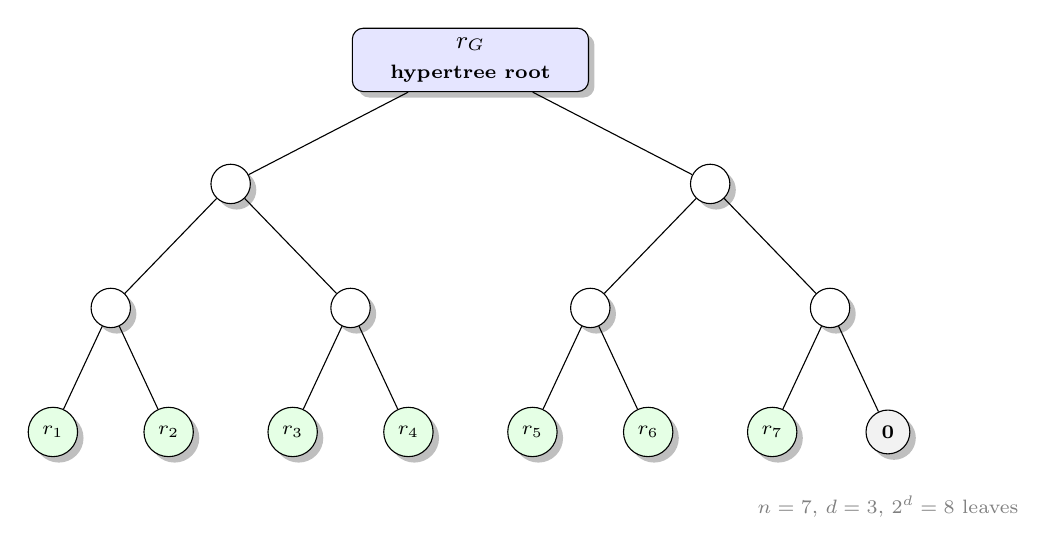
\begin{tikzpicture}[
    scale=1.05,
    level distance=1.5cm,
    level 1/.style={sibling distance=5.8cm},
    level 2/.style={sibling distance=2.9cm},
    level 3/.style={sibling distance=1.4cm},
    every node/.style={font=\small},
  ]

  %% --- 5-of-7 group, depth 3 ------------------------------------
  \node[root box] (root) {$r_G$\\\scriptsize hypertree root}
    child {
      node[leaf node, fill=white!10] (A) {}
      child {
        node[leaf node, fill=white!10] (C) {}
        child { node[leaf node] (l1) {$r_1$} }
        child { node[leaf node] (l2) {$r_2$} }
      }
      child {
        node[leaf node, fill=white!10] (D) {}
        child { node[leaf node] (l3) {$r_3$} }
        child { node[leaf node] (l4) {$r_4$} }
      }
    }
    child {
      node[leaf node, fill=white!10] (B) {}
      child {
        node[leaf node, fill=white!10] (E) {}
        child { node[leaf node] (l5) {$r_5$} }
        child { node[leaf node] (l6) {$r_6$} }
      }
      child {
        node[leaf node, fill=white!10] (F) {}
        child { node[leaf node] (l7) {$r_7$} }
        child { node[leaf node, fill=gray!10] (l8) {$\mathbf{0}$} }
      }
    };
    
  %% legend
  \node[below=0.4cm of l8, font=\scriptsize, gray]
    {$n=7$, $d=3$, $2^d = 8$ leaves};
\end{tikzpicture}
\caption{Hypertree for a $x$-out-of-7 threshold group ($n=7$, depth $d=3$). Seven $\XMSS$ public keys $r_1,\ldots,r_7$ are placed as leaves; the eighth leaf is zero-padded.  Each internal node is a $\poseidon_{16}$ compression of its two children. The hypertree root $r_G$ is the joint public key appearing in the global \texttt{pub\_keys} list.}
\label{fig:hypertree}
\end{figure}

\noindent While Definition~\ref{def:thresh_group} is generic regardless of the $k$ and $n$ parameters, we hereafter assume $n \leq 8$ as distributed validators rarely exceed 8 participants.
Indeed most configurations use either $(k,n) = (3,4)$ or $(5,7)$. 
A threshold signature then consists of a set of signer indices, individual signatures and membership proofs as defined hereafter. 

\begin{definition}[Threshold Signature]
  Given a group $G = (k, n, \hypertree)$ and a message $m$, a threshold signature is a tuple $\Sigma = (\mathbf{i}, \boldsymbol{\sigma}, \boldsymbol{\pi})$ where:
  \begin{itemize}
    \item[-] $\mathbf{i} = (i_1, \ldots, i_k)$ is a set of $k$ distinct signer indices, $i_j \in \{1, \ldots, n\}$.
    \item[-] $\boldsymbol{\sigma} = (\sigma_1, \ldots, \sigma_k)$ are the $k$ individual $\XMSS$ signatures, $\sigma_j$ being the signature of signer $i_j$ on $m$.
    \item[-] $\boldsymbol{\pi} = (\pi_1, \ldots, \pi_k)$ are the corresponding Merkle authentication paths, where $\pi_j$ contains the $d$ sibling hashes required to reconstruct the root $r_G$ from the leaf $r_{i_j}$.
  \end{itemize}
\end{definition}

\bigskip
\noindent Threshold signature verification consists of three independent checks per signer:
\begin{enumerate}
  \item \textbf{XMSS validity}: $\XMSS.\mathsf{Verify}(r_{i_j}, m, \sigma_j) = \top$.
  \item \textbf{Hypertree membership}: the Merkle path $\pi_j$ successfully authenticates the leaf $r_{i_j}$ against the known joint public key $r_G$.
  \item \textbf{Distinctness}: no index $i_j$ appears more than once in $\mathbf{i}$.
\end{enumerate}

\noindent The combined verification cost is dominated by the $k$ $\XMSS$ verifications, each requiring $O(V \cdot L + \log_{\text{lifetime}})$ \poseidon calls (WOTS chains + \XMSS Merkle path), plus $k \times d$ additional \poseidon calls for the hypertree paths.


% ═══════════════════════════════════════════════════════════════════════════════
\section{Integration of Threshold Signatures into leanVM}
% ═══════════════════════════════════════════════════════════════════════════════

\subsection{Overview}
The most straightforward way to extend \leanVM in order to support dummy threshold signatures is to perform the verification of all $k$ signers in a threshold group \emph{inside the same aggregation circuit} as the raw \XMSS and recursive proof checks.
It implies supporting threshold signatures as a new source type in \texttt{main.py}, processed between raw \XMSS and recursive sources.
%\begin{observation}[Constant overhead of dummmy threshold signatures]
Unlike proof-based threshold signatures, the dummy threshold verification logic (\XMSS verification of each signer plus $d \leq 3$ additional \poseidon hashes per signer for the hypertree path) is added as extra rows in the execution trace, not as an additional proof system invocation.  The proving cost of extra trace rows is sublinear (only log factors enter through \WHIR), so a threshold group with $k = 7$ signers adds roughly the same overhead as $7$ extra raw \XMSS signatures.
%\end{observation}
\noindent Beyond the raw cost argument, it has the advantage to keep a single bytecode program and an homogeneous recursion interface as no new proof type is introduced.

\subsection{In-Circuit Threshold Verification}

The in-circuit implementation lives in \texttt{threshold\_aggregate.py} and is compiled into the same bytecode as the rest of \texttt{main.py}.

\subsubsection{Private Input Layout}

Each threshold source block in private memory has the layout:
\[
  \underbrace{k}_{\text{threshold}}\;\;
  \underbrace{d}_{\text{depth}}\;\;
  \underbrace{j}_{\text{pubkey idx}}\;\;
  \underbrace{\ell_1, \ldots, \ell_k}_{\text{leaf indices}}\;\;
  \underbrace{r_{\ell_1}, \ldots, r_{\ell_k}}_{\text{signer roots (hints)}}\;\;
  \underbrace{\sigma_1, \ldots, \sigma_k}_{\text{XMSS sigs}}\;\;
  \underbrace{\pi_1, \ldots, \pi_k}_{\text{hypertree proofs}}
\]
where each signer root $r_{\ell_i} \in \KB^8$ is provided as a private hint (not trusted; it is recomputed and verified in-circuit), and each hypertree proof $\pi_i$ consists of $d$ sibling digests.

The global private input header was extended from the pre-threshold format:
\begin{center}
\resizebox{\textwidth}{!}{
\begin{tabular}{ll}
\toprule
Layout & Description \\ \midrule
\texttt{[n\_recursions]} & Number of recursive child proofs \\
\texttt{[n\_threshold]} & Number of threshold source blocks \\
\texttt{[n\_dup]} & Number of duplicate public keys \\
\texttt{[ptr\_pubkeys]} & Pointer to global public key table \\
\texttt{[ptr\_src\_0, ptr\_thresh\_0..t, ptr\_rec\_0..n, ptr\_bytecode\_sumcheck]}
  & Ordered source pointers \\ \bottomrule
\end{tabular}
}
\end{center}

\subsubsection{Verification Algorithm}

For each threshold source block (indexed $t = 0, \ldots, n_{\text{threshold}} - 1$), the circuit executes Algorithm~\ref{alg:threshold-verify}.

\begin{algorithm}[H]
\caption{\texttt{threshold\_verify\_group} (in-circuit, zkDSL)}
\label{alg:threshold-verify}
\begin{algorithmic}[1]
\Require $k$: threshold; $d$: depth; $j$: global pubkey index;
         $\ell_1,\ldots,\ell_k$: leaf indices;
         $r_{\ell_i}$: signer root hints;
         $\sigma_i$: XMSS signatures;
         $\pi_i$: hypertree proofs ($d$ siblings each)
\State $r_G \gets \texttt{all\_pubkeys}[j]$ \quad\Comment{expected hypertree root (public)}
\State $\texttt{seen} \gets \texttt{Array}(2^d)$ \quad\Comment{write-once bitmap for distinctness}
\For{$i = 0 \to k-1$}
  \State Assert $\ell_i < 2^d$ \quad\Comment{leaf index in bounds}
  \State $\texttt{seen}[\ell_i] \gets i + 1$
    \quad\Comment{write-once: duplicate $\ell_i$ triggers MemoryAlreadySet}
  \State $\XMSS.\mathsf{InCircuitVerify}(r_{\ell_i},\; m,\; \sigma_i,\; \text{slot})$
    \quad\Comment{writes $r_{\ell_i}$ to its hint address; memory-write assertion}
  \State $\hat{r}_G \gets \texttt{HypertreeMerkleVerify}(r_{\ell_i}, \pi_i, \ell_i, d)$
  \State Assert $\hat{r}_G = r_G$ element-wise \quad\Comment{explicit equality check}
\EndFor
\State \Return $j$ \quad\Comment{global pubkey index used for partition counter}
\end{algorithmic}
\end{algorithm}

\subsubsection{Distinctness via Write-Once Memory}

The bitmap array \texttt{seen[MAX\_THRESHOLD\_SIGNERS]} uses the write-once memory property of \leanVM to enforce signer index uniqueness without a sorting circuit or a hash set.  On the first write, \texttt{seen}[$\ell_i$] $\gets i+1$ succeeds.  On a second write with any other value (since $i$ is strictly increasing), the memory constraint
\[
  \text{(previous value)} = \text{(new value)}
\]
is violated, causing an unsatisfiable AIR constraint.  This is provably sound under the Logup bus argument: the memory table enforces that every read is consistent with the unique write that created the entry.

\subsubsection{Hypertree Merkle Verification (Depth Dispatch)}

Because the maximum depth is $d \leq 3$ and is known at compile time from the \texttt{MAX\_HYPERTREE\_DEPTH} placeholder, the circuit dispatches statically on $d$ rather than using a variable-depth loop:

\begin{lstlisting}[style=zkdsl, caption={Depth dispatch in \texttt{threshold\_aggregate.py}}]
@inline
def hypertree_merkle_verify(leaf_digest, proof_path, leaf_idx, depth, out_root):
    match depth:
        case 1: _hypertree_verify_d1(leaf_digest, proof_path, leaf_idx, out_root)
        case 2: _hypertree_verify_d2(leaf_digest, proof_path, leaf_idx, out_root)
        case 3: _hypertree_verify_d3(leaf_digest, proof_path, leaf_idx, out_root)
    return
\end{lstlisting}

Each \texttt{\_hypertree\_verify\_d} function is a fixed chain of $\poseidon_{16}$ calls with a \texttt{match} on the bit decomposition of \texttt{leaf\_idx}.  The bit decomposition is \emph{big-endian}: bit index $\texttt{depth}-1-j$ controls the direction (left/right) at Merkle level $j$ (counted from the leaves).  Left child means $b=0$: $\poseidon(\texttt{current}, \texttt{sibling})$; right child means $b=1$: $\poseidon(\texttt{sibling}, \texttt{current})$.
See Listing~\ref{lst:depth3} for an example with depth 3.

\begin{lstlisting}[style=zkdsl, caption={Depth-3 Merkle verification}, label=lst:depth3]
def _hypertree_verify_d3(leaf_digest, proof, leaf_idx, out_root):
    bits = checked_decompose_bits_small_value_const(leaf_idx, 3)  # [MSB, mid, LSB]
    temp0 = Array(DIGEST_LEN)
    temp1 = Array(DIGEST_LEN)
    match bits[2]:   # level 0 (leaves): LSB
        case 0: poseidon16(leaf_digest, proof,             temp0)
        case 1: poseidon16(proof,        leaf_digest,      temp0)(
    match bits[1]:   # level 1
        case 0: poseidon16(temp0, proof + DIGEST_LEN,     temp1)
        case 1: poseidon16(proof + DIGEST_LEN, temp0,     temp1)
    match bits[0]:   # level 2 (root's children): MSB
        case 0: poseidon16(temp1, proof + 2*DIGEST_LEN,   out_root)
        case 1: poseidon16(proof + 2*DIGEST_LEN, temp1,   out_root)
    return
\end{lstlisting}

\subsubsection{Root Assertion Pattern}

A subtle correctness point: the signer root $r_{\ell_i}$ passed into \texttt{xmss\_verify} is a \emph{hint} in the private input at a known address.  The $\XMSS$ circuit writes the re-derived root to that address via the memory-write assertion.  The hypertree circuit then reads that same address to begin the Merkle path computation.

The hypertree root $\hat{r}_G$ is computed into a \emph{fresh} buffer (not into the \texttt{all\_pubkeys} region), because that region may already have been written.  An explicit element-wise assertion
\[
  \hat{r}_G[j] = r_G[j], \quad j = 0, \ldots, 7
\]
is emitted rather than relying on the write-once memory assertion pattern. This design choice makes correctness independent of the memory state of \texttt{all\_pubkeys}.

\subsection{Poseidon Precomputation}
\label{subsec:poseidon-precomp}

The \leanProver requires all $\poseidon_{16}$ input--output pairs to be provided before trace generation (the $\poseidon_{16}$ table is populated from hints, not re-evaluated in the execution trace).  For threshold signatures, each signer contributes:
\begin{itemize}
  \item All \poseidon calls from WOTS chain evaluation and XMSS Merkle path.
  \item $d \leq 3$ additional \poseidon calls for the hypertree path.
\end{itemize}
The function \texttt{threshold\_verify\_with\_poseidon\_trace} in
\texttt{crates/xmss/src/hypertree.rs} performs native verification while
collecting the full trace:

\begin{lstlisting}[language=Rust, style=boxed,
  caption={Trace collection for hypertree path (Rust, \texttt{hypertree.rs})}]
for sibling in &proof {
    let is_left = (idx & 1) == 0;
    current = if is_left {
        poseidon16_compress_with_trace(&current, sibling, &mut poseidon_trace)
    } else {
        poseidon16_compress_with_trace(sibling, &current, &mut poseidon_trace)
    };
    idx >>= 1;
}
\end{lstlisting}

All threshold \poseidon traces are parallelised over groups with Rayon, then
merged with the raw XMSS traces before being passed to
\texttt{prove\_execution}.

%\subsection{End-to-End Aggregation with Threshold Groups}
%\label{subsec:e2e}
%
%Figure~\ref{fig:e2e} shows a multi-level aggregation tree where leaf nodes
%handle raw XMSS signatures and threshold groups, and a root node aggregates
%their proofs recursively.
%
%\begin{figure}[H]
%\centering
%\begin{tikzpicture}[node distance=1.1cm and 1.4cm]
%
%  %% Leaf 1: raw XMSS only
%  \node[proof node, fill=green!15] (L1) at (-5.5, 0) {$\pi_1$};
%  \node[leaf node, above left=0.7cm and 0.1cm of L1]  (r11) {$\sigma_1$};
%  \node[leaf node, above right=0.7cm and 0.1cm of L1] (r12) {$\sigma_2$};
%  \draw[arr] (r11) -- (L1);
%  \draw[arr] (r12) -- (L1);
%  \node[font=\scriptsize, below=0.2cm of L1] {Raw XMSS leaf};
%
%  %% Leaf 2: threshold group
%  \node[proof node, fill=orange!20] (L2) at (-0.5, 0) {$\pi_2$};
%  \node[thresh node, above left=0.7cm and 0.0cm of L2] (t1) {$G_1$\\5-of-7};
%  \node[leaf node, above right=0.7cm and 0.0cm of L2] (r21) {$\sigma_3$};
%  \draw[arr] (t1)  -- (L2);
%  \draw[arr] (r21) -- (L2);
%  \node[font=\scriptsize, below=0.2cm of L2] {Threshold + Raw leaf};
%
%  %% Leaf 3: another threshold group
%  \node[proof node, fill=orange!20] (L3) at (4.5, 0) {$\pi_3$};
%  \node[thresh node, above left=0.7cm and 0.0cm of L3] (t2) {$G_2$\\3-of-5};
%  \node[leaf node, above right=0.7cm and 0.0cm of L3] (r31) {$\sigma_4$};
%  \draw[arr] (t2)  -- (L3);
%  \draw[arr] (r31) -- (L3);
%  \node[font=\scriptsize, below=0.2cm of L3] {Threshold + Raw leaf};
%
%  %% Root
%  \node[root box] (Root) at (0, -2.4) {$\pi_{\text{root}}$\\($n = 2 + 1 + r_G + r_{G'} + \ldots$ pubkeys)};
%  \draw[arr] (L1) -- (Root) node[midway, sloped, font=\scriptsize, above]{rec. child};
%  \draw[arr] (L2) -- (Root) node[midway, sloped, font=\scriptsize, above]{rec. child};
%  \draw[arr] (L3) -- (Root) node[midway, sloped, font=\scriptsize, above]{rec. child};
%
%  \node[font=\scriptsize, gray, below=0.15cm of Root]
%    {One SNARK: constant proof size, independent of total validator count};
%\end{tikzpicture}
%\caption{Multi-level aggregation tree with threshold groups.
%         Leaf nodes (orange) embed threshold group verification inline.
%         The root aggregation node verifies all three child proofs
%         recursively.  The final proof $\pi_{\text{root}}$ is constant-size
%         regardless of the total number of validators.}
%\label{fig:e2e}
%\end{figure}
%
%\subsection{Comparison with the Proof-Based Approach}
%\label{subsec:comparison}
%
%The \texttt{threshold\_main.py} program is a standalone circuit for
%producing a \texttt{ThresholdAggregatedSig} artifact without embedding the
%threshold group in a larger aggregation.  Its public input layout is:
%\[
%  \underbrace{r_G}_{\text{thresh. root}}\;\;
%  \underbrace{k_{\min}}_{\text{min. signers}}\;\;
%  \underbrace{m}_{\text{message}}\;\;
%  \underbrace{\text{slot}_{lo}, \text{slot}_{hi}}_{\text{slot range}}\;\;
%  \underbrace{\text{merkle\_chunks}}_{\text{XMSS param}}\;\;
%  \underbrace{\text{bytecode\_claim}}_{\text{self-referential}}
%\]
%The minimum-signer count $k_{\min}$ is committed to the public input,
%allowing verifiers to enforce the group policy without knowing the full
%private input.
%
%While this standalone circuit is useful for proving threshold policies
%independently of any parent aggregation, its use as a sub-proof in
%Approach~B imposes the following penalties (measured in the
%\texttt{inline-vs-recursive-threshold} benchmark):
%
%\begin{center}
%\begin{tabular}{lcc}
%\toprule
%Metric & Approach A (inline) & Approach B (recursive) \\ \midrule
%Proofs generated & 1 & 2 \\
%Wall-clock time (5-of-7) & $t_{\text{leaf}}$ & $t_{\text{leaf}} + t_{\text{parent}} \approx 1.8\text{--}2.0 \times t_{\text{leaf}}$ \\
%Extra proving cycles & 0 & $\sim 10^6$ (parent recursion) \\
%Extra proof overhead & 0 & $+$200--400 KiB (parent proof) \\
%API complexity & simple & new proof type + pipeline stage \\
%\bottomrule
%\end{tabular}
%\end{center}
%
%The $t_{\text{parent}}$ overhead exists because the parent circuit must
%execute the full recursion verifier in zkDSL --- including WHIR
%decommitment verification, Logup argument checks, and SuperSpartan
%sumcheck verification --- over the child's proof transcript.  This is
%a fixed cost that scales with the size of the child's SNARK, not with the
%number of signers.  Since the recursion verifier is the most
%computationally expensive part of the aggregation circuit, using a full
%proof layer for each threshold group is impractical when many groups are
%present.

% ═══════════════════════════════════════════════════════════════════════════════
\section{Implications for Distributed Validators}
\label{sec:dv}
% ═══════════════════════════════════════════════════════════════════════════════

\subsection{Key Registration}
\label{subsec:key-reg}

In the pre-quantum DV model, an operator cluster registers a single BLS key on the Ethereum beacon chain.  Under \leanConsensus, the registration changes: the cluster registers the \emph{hypertree root} $r_G$ along with the threshold parameters $(k,n)$.  This root is a 248-bit hash-based commitment to all $n$ members' $\XMSS$ public keys.
The hypertree is constructed off-chain by any cluster member (or a trusted coordinator) as:
\begin{enumerate}
  \item Each node independently generates an $\XMSS$ key pair  $(sk_i, pk_i)$ with $pk_i = r_i \in \KB^8$.
  \item All $n$ roots $r_1, \ldots, r_n$ are shared to all nodes that are part of the DV cluster.
  \item Any member computes $\hypertree$ and the joint key $r_G = \hypertree.\mathsf{Root}$.
  \item $r_G$ is submitted for registration as the joint public key.
\end{enumerate}

No trusted dealer is required, and no secret is shared between operators: each holds only their own $\XMSS$ key.

\subsection{Signing Protocol}
\label{subsec:signing-protocol}

During operation, the signing protocol for a slot $s$ proceeds as:
\begin{enumerate}
  \item The consensus layer broadcasts the message $m$ (e.g., an attestation
        beacon block root) and slot $s$.
  \item Each of the $n$ reachable operators independently signs:
        $\sigma_i \gets \XMSS.\mathsf{Sign}(sk_i, m, s)$.
  \item A designated \emph{aggregator} (possibly rotating) collects at
        least $k$ valid signatures.
  \item The aggregator constructs $\Sigma = (\mathbf{i}, \boldsymbol{\sigma})$
        and calls \texttt{aggregate([], [], [(G, sigma)], m, s)}.
  \item The resulting \texttt{AggregatedSigs} is submitted to the Ethereum
        consensus layer (or to a parent aggregation node).
\end{enumerate}

The $\XMSS$ signing operations are entirely independent and can proceed in
parallel.  The only sequential step is proof generation, which takes
$O(k)$ XMSS verification costs in the circuit.
%
%\subsection{Slashing Protection}
%\label{subsec:slashing}
%
%$\XMSS$ is stateful: each slot index can only be signed once.  Signing the
%same slot twice (double-voting) risks equivocation.  In a DV cluster, each
%operator manages their own $\XMSS$ state (the slot counter).  Since operators
%are independent, there is no risk of one operator causing another's key to
%be reused.
%
%However, the \emph{aggregator} must enforce that no operator submits two
%different signatures for the same slot.  The circuit does not prevent
%this by itself --- it verifies whatever XMSS signatures are provided.
%Slashing protection must be implemented at the protocol layer (e.g., by
%having operators only sign messages received through an authenticated
%consensus channel).
%
%\subsection{Security Model}
%\label{subsec:security-model}
%
%\begin{definition}[k-of-n Security]
%  A threshold group $G = (k, n, \hypertree)$ is \emph{$k$-of-$n$ secure}
%  if: (i) any adversary controlling fewer than $k$ operators cannot produce
%  a valid threshold signature $\Sigma$; (ii) any subset of $k$ honest
%  operators can always produce a valid $\Sigma$.
%\end{definition}
%
%Property (i) follows from the existential unforgeability of $\XMSS$:
%forging a signature $\sigma_i$ without the corresponding $sk_i$ requires
%breaking the one-wayness of $\poseidon$, which is post-quantum secure under
%the quantum random oracle model.  Property (ii) holds by construction, since
%$k$ independent signers can always collect their $\XMSS$ signatures.
%
%The in-circuit distinctness check (via the write-once bitmap) prevents an
%adversary from counting the same signer twice to reach the threshold.
%The hypertree Merkle proof check prevents claiming that a forged XMSS key
%belongs to the group.  Together, these constraints mean that the only way
%to produce a valid threshold proof is to hold at least $k$ distinct private
%$\XMSS$ keys whose public key digests are leaves of $\hypertree$.

% ═══════════════════════════════════════════════════════════════════════════════
\section{Open Challenges for Distributed Validator Deployment}
\label{sec:challenges}
% ═══════════════════════════════════════════════════════════════════════════════

\subsection{Cluster Mutability and Key Rotation}
\label{subsec:mutability}

\paragraph{The problem.}
The hypertree root $r_G$ is a static commitment to $n$ specific $\XMSS$ public keys.  Once $r_G$ is registered on-chain, it cannot be updated without a new on-chain transaction.  Real DV clusters need to handle:
\begin{itemize}
  \item \emph{Member churn}: an operator leaves and is replaced.
  \item \emph{Key rotation}: an operator suspects key compromise and generates a fresh $\XMSS$ key pair.
  \item \emph{Threshold adjustment}: the cluster policy changes (e.g., from 3-of-5 to 4-of-5 after detecting an unreliable member).
\end{itemize}

\paragraph{Current limitation.}
The current implementation has no on-chain mechanism for updating $r_G$.
A cluster that needs to change membership must:
\begin{enumerate}
  \item Generate a new hypertree $\hypertree'$ with updated members.
  \item Submit an exit transaction for the old validator (identified by $r_G$).
  \item Register a new validator with the new joint key $r_G'$.
\end{enumerate}
This process requires waiting for the exit queue and incurs a new deposit.

%\paragraph{Potential mitigations.}
%One direction is a \emph{hierarchical hypertree} with a mutable member list.
%For instance, a top-level hypertree could commit to a set of \emph{delegation roots}, where each delegation root is itself the root of a smaller hypertree.
%Key rotation within a delegation would only require updating one leaf of the top-level tree, but the on-chain registration (the top-level root) would need to be updated.
%
%A more radical approach uses a hash-based \emph{updatable commitment}: the on-chain registration stores not $r_G$ directly but a hash chain over versioned hypertree roots.
%Updating the tree produces a new version, and valid proofs for any version in the chain are accepted.
%This requires protocol-level changes to the Ethereum validator registration.
%
%A third approach decouples the identity commitment from the signing key: the on-chain identity is an abstract identifier (e.g., a smart contract address), and the current $\XMSS$ public keys are published in a separate registry.
%Signers prove membership in the current registry rather than in a fixed tree.
%This requires a different circuit design (proving registry inclusion rather than hypertree membership) and a trust model for the registry.

%\subsection{Aggregator Role and Incentives}
%\label{subsec:aggregator}
%
%The aggregator collects signatures from operators and generates the SNARK proof.
%In the current design, this is a centralised role with no redundancy.  If the
%aggregator fails, no proof is submitted for that slot.  Production deployment
%requires:
%\begin{itemize}
%  \item \emph{Redundant aggregators}: multiple candidates attempt aggregation;
%        the first valid proof is accepted.
%  \item \emph{Incentive alignment}: the aggregator must be compensated for
%        proof generation costs ($O(\text{minutes})$ of computation for a
%        leaf-level proof with $k = 7$ XMSS verifications).
%  \item \emph{Aggregator censorship resistance}: if the designated aggregator
%        is malicious and refuses to include certain operators' signatures, the
%        cluster may fall below threshold despite having enough honest operators.
%\end{itemize}
%
%\subsection{Proof Latency vs. Slot Time}
%\label{subsec:latency}
%
%Ethereum's slot time is 12 seconds.  The attestation deadline is 4 seconds.
%Generating a leaf-level SNARK proof with $k = 7$ XMSS verifications currently
%takes several tens of seconds on commodity hardware (depending on the WHIR
%code rate and the number of grinding bits).  This is far too slow for
%real-time attestation.
%
%Several approaches to close this gap are being explored:
%\begin{itemize}
%  \item \emph{Pre-aggregation}: proof generation can start as soon as $k$
%        signatures are collected, before the attestation deadline, if the
%        message is known in advance (e.g., block proposals are known early).
%  \item \emph{Hardware acceleration}: FPGA/GPU backends for Poseidon hashing
%        and polynomial arithmetic.
%  \item \emph{Proof caching and amortisation}: proofs for the same slot's
%        attestation can be shared across multiple aggregation trees.
%  \item \emph{Async submission}: submit the aggregated proof asynchronously,
%        using a delayed settlement protocol (e.g., an optimistic layer that
%        accepts delayed proofs and penalises dishonest claims).
%\end{itemize}
%
%\subsection{Upgradeability of the SNARK Circuit}
%\label{subsec:upgradeability}
%
%The bytecode of \texttt{main.py} is compiled at deployment time and fixed.
%Its hash is committed via the self-referential compilation loop.  If a bug
%is found in the circuit or if XMSS parameters must change (e.g., $V$, $W$,
%or \texttt{LOG\_LIFETIME}), all on-chain validators must coordinate a
%migration:
%\begin{itemize}
%  \item A new bytecode is compiled with updated parameters.
%  \item A ``migration epoch'' is agreed upon.
%  \item All nodes re-prove their signatures using the new circuit.
%\end{itemize}
%This is analogous to a hard fork in the proof system.  Ideally, the
%circuit should be versioned, and the on-chain verifier should accept proofs
%from any authorised version.  This requires an on-chain registry of valid
%bytecodes and corresponding verifier keys.
%
%\subsection{Maximum Group Size and Weighted Thresholds}
%\label{subsec:group-size}
%
%The current implementation caps the hypertree depth at 3, limiting group size
%to $n \leq 8$.  For larger DV clusters (e.g., institutional validators with
%$n = 21$ or $n = 100$ members), this is insufficient.
%
%Extending to depth 4 ($n \leq 16$) or depth 5 ($n \leq 32$) requires adding
%new \texttt{\_hypertree\_verify\_d4} / \texttt{\_hypertree\_verify\_d5} cases to
%\texttt{threshold\_aggregate.py}.  For very large $n$, the static dispatch
%becomes unwieldy; a dynamic unroll (as used in the XMSS Merkle verification)
%should replace it.
%
%Additionally, the current design treats all members equally: each member
%contributes 1 unit toward the threshold.  Institutional DV clusters may
%want \emph{weighted thresholds} where high-reputation or high-stake
%operators have more voting power.  This requires replacing the signer count
%$k$ with a weighted sum $\sum_{i \in \mathbf{i}} w_i \geq k_{\text{min}}$,
%where weights $w_i$ are committed in the hypertree leaves or in a separate
%table.
%
%\subsection{Formal Security Proofs}
%\label{subsec:formal-security}
%
%The system's security rests on several unproven assumptions:
%\begin{itemize}
%  \item The combination of SuperSpartan + WHIR + Logup is sound for the
%        specific circuit structure used (three table types, specific AIR
%        degrees).  The individual protocols have security proofs, but
%        their composition has not been formally analysed in the combined
%        setting.
%  \item The self-referential compilation loop converges to the correct
%        bytecode.  This is asserted by the convergence test in
%        \texttt{compile\_main\_program\_self\_referential} but not formally
%        proved.
%  \item The threshold security of the inline verification is sound under
%        the write-once memory model of \leanVM.  A formal reduction from
%        threshold security to the one-wayness of $\poseidon$ would be
%        desirable.
%\end{itemize}
%
%% ═══════════════════════════════════════════════════════════════════════════════
%\section{Conclusion}
%\label{sec:conclusion}
%% ═══════════════════════════════════════════════════════════════════════════════
%
%\leanConsensus{} provides a post-quantum, hash-based aggregation system for
%Ethereum validator signatures that natively supports DV clusters through the
%hypertree construction.  The inline threshold verification strategy avoids the
%$\approx 2\times$ proving overhead of the recursive sub-proof strategy, making
%the system practical for DV clusters of up to 8 members with a single-circuit
%design.
%
%The main engineering challenges remaining before live deployment are:
%cluster mutability (key rotation and member churn without on-chain
%re-registration), proof latency (closing the gap between proving time and
%the 12-second Ethereum slot time), aggregator redundancy, and formal security
%proofs for the composite protocol.  These are active areas of research and
%development within the Obol Network.

% ─── bibliography ─────────────────────────────────────────────────────────────
\bibliographystyle{alpha}
\bibliography{bib}

\end{document}
